\documentclass{article}
\usepackage{amsmath}
\usepackage{amsfonts}
\usepackage{graphicx}
\title{Machine Learning lecture notes}
\author{Khoa Hoang Viet \thanks{based on Andrew Ng's Machine Learning course in coursera.org}}
\date{\today}
\begin{document}
\section{Classification and Representation}
\subsection{Classification}
The \textbf{classification problem} is just like the regression problem, except that \textit{the values we now want to predict take on only a small number of discrete values.} 

For now, we will focus on the binary classification problem in which y can take on only two values, 0 and 1. (Most of what we say here will also generalize to the multiple-class case.) For instance, if we are trying to build a spam classifier for email, then $x^{(i)}$ may be some features of a piece of email, and y may be 1 if it is a piece of spam mail, and 0 otherwise. Hence, $y \in\{0, 1\}$.

0 is also called the negative class, and 1 the positive class, and they are sometimes also denoted by the symbols “-” and “+.” Given $x^{(i)}$, the corresponding $y^{(i)}$ is also called the label for the training example.

To attempt classification, one method is to use linear regression and map all predictions greater than 0.5 as a 1 and all less than 0.5 as a 0. However, this method doesn't work well because classification is not actually a linear function.

\textbf{Logistic Regression} is a classification algorithm that we apply to settings where the label y is discrete value, when it's either zero or one. 

Don't be confused by the name \textbf{"Logistic Regression"}; it is named that way for historical reasons and is actually an approach to classification problems, not regression problems.


\subsection{Hypothesis Representation}
We could approach the classification problem ignoring the fact that y is discrete-valued, and use our old linear regression algorithm to try to predict y given x. However, it is easy to construct examples where this method performs very poorly.

Intuitively, it also doesn’t make sense for $h_\theta (x)$ to take values larger than 1 or smaller than 0 when we know that $y \in\{0, 1\}$.

To fix this, let’s change the form for our hypotheses $h_\theta (x)$ to satisfy $0 \leq h_\theta (x) \leq 1$. This is accomplished by plugging $\theta^Tx$ into the Logistic Function.

Our new form uses the \textbf{"Sigmoid Function}," also called the \textbf{"Logistic Function"}:
\begin{align*}
	& h_\theta (x) = g ( \theta^T x ) \\ 
	& z = \theta^T x \\
	& g(z) = \dfrac{1}{1 + e^{-z}}
\end{align*}

The following image shows us what the sigmoid function looks like:\\
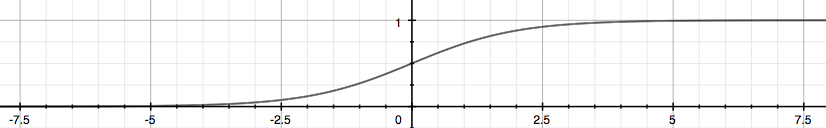
\includegraphics[width=\textwidth]{Logistic_function}

The function g(z), shown here, maps any real number to the (0, 1) interval, making it useful for transforming an arbitrary-valued function into a function better suited for classification.

$h_\theta(x)$ will give us the probability that our output is 1. For example, $h_\theta(x)=0.7$ gives us a probability of 70\% that our output is 1. Our probability that our prediction is 0 is just the complement of our probability that it is 1 (e.g. if probability that it is 1 is 70\%, then the probability that it is 0 is 30\%).

\begin{align*}
	& h_\theta(x) = P(y=1 | x ; \theta) = 1 - P(y=0 | x ; \theta) \\
	& P(y = 0 | x;\theta) + P(y = 1 | x ; \theta) = 1
\end{align*}

\subsection{Decision Boundary}
In order to get our discrete 0 or 1 classification, we can translate the output of the hypothesis function as follows:
\begin{align*}
	&h_\theta(x) \geq 0.5 \rightarrow y = 1 \\
	&h_\theta(x) < 0.5 \rightarrow y = 0 \\
\end{align*}

The way our logistic function g behaves is that when its input is greater than or equal to zero, its output is greater than or equal to 0.5:
\begin{align*}
	& g(z) \geq 0.5 \\
	& when \; z \geq 0
\end{align*}

Remember.
\begin{align*}
	z=0, e^{0}=1 \Rightarrow g(z)=1/2\\ 
	z \to \infty, e^{-\infty} \to 0 \Rightarrow g(z)=1 \\ 
	z \to -\infty, e^{\infty}\to \infty \Rightarrow g(z)=0 
\end{align*}

So if our input to g is $\theta^T X$, then that means:
\begin{align*}
	& h_\theta(x) = g(\theta^T x) \geq 0.5 \\
	& when \; \theta^T x \geq 0
\end{align*}

From these statements we can now say:
\begin{align*}
	& \theta^T x \geq 0 \Rightarrow y = 1 \\
	& \theta^T x < 0 \Rightarrow y = 0 \\
\end{align*}
The \textbf{decision boundary} is the line that separates the area where y = 0 and where y = 1. It is created by our hypothesis function.

\textbf{Example:}
\begin{align*}
	& \theta = \begin{bmatrix}5 \\ -1 \\ 0\end{bmatrix} \\ 
	& y = 1 \; if \; 5 + (-1) x_1 + 0 x_2 \geq 0 \\ 
	& 5 - x_1 \geq 0 \\ & - x_1 \geq -5 \\
	& x_1 \leq 5 \\ 
\end{align*}

In this case, our decision boundary is a straight vertical line placed on the graph where $x_1 = 5$, and everything to the left of that denotes y = 1, while everything to the right denotes y = 0.

Again, the input to the sigmoid function g(z) (e.g. $\theta^T X$) doesn't need to be linear, and could be a function that describes a circle (e.g. $z = \theta_0 + \theta_1 x_1^2 +\theta_2 x_2^2$) or any shape to fit our data.

\section{Logistic Regression Model}
\subsection{Cost Function}
We cannot use the same cost function that we use for linear regression because the Logistic Function will cause the output to be wavy, causing many local optima. In other words, it will not be a convex function.

Instead, our cost function for logistic regression looks like:
\begin{align*}
	& J(\theta) = \dfrac{1}{m} \sum_{i=1}^m \mathrm{Cost}(h_\theta(x^{(i)}),y^{(i)}) \\ 
	& \mathrm{Cost}(h_\theta(x),y) = -\log(h_\theta(x)) \; & \text{if y = 1} \\
	& \mathrm{Cost}(h_\theta(x),y) = -\log(1-h_\theta(x)) \; & \text{if y = 0}
\end{align*}

When y = 1, we get the following plot for $J(\theta)$ vs $h_\theta (x)$:\\
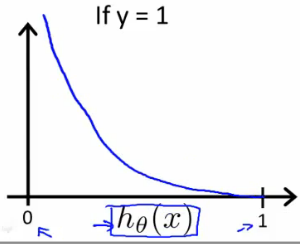
\includegraphics{Logistic_regression_cost_function_positive_class}

Similarly, when y = 0, we get the following plot for $J(\theta)$ vs $h_\theta (x)$:\\
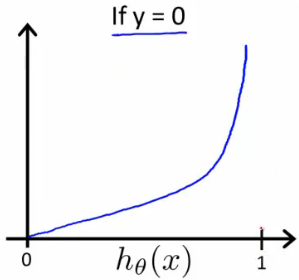
\includegraphics{Logistic_regression_cost_function_negative_class}

\begin{align*}
	& \mathrm{Cost}(h_\theta(x),y) = 0 \text{ if } h_\theta(x) = y \\ 
	& \mathrm{Cost}(h_\theta(x),y) \rightarrow \infty \text{ if } y = 0 \; \mathrm{and} \; h_\theta(x) \rightarrow 1 \\ 
	& \mathrm{Cost}(h_\theta(x),y) \rightarrow \infty \text{ if } y = 1 \; \mathrm{and} \; h_\theta(x) \rightarrow 0 \newline 
\end{align*}

If our correct answer 'y' is 0, then the cost function will be 0 if our hypothesis function also outputs 0. If our hypothesis approaches 1, then the cost function will approach infinity.

If our correct answer 'y' is 1, then the cost function will be 0 if our hypothesis function outputs 1. If our hypothesis approaches 0, then the cost function will approach infinity.

Note that writing the cost function in this way guarantees that J(θ) is convex for logistic regression.

\end{document}
